\documentclass[11pt,a4paper,oldfontcommands]{memoir}
\usepackage[utf8]{inputenc}
\usepackage[T1]{fontenc}
\usepackage{microtype}
\usepackage[dvips]{graphicx}
\usepackage{xcolor}
\usepackage{times}
\usepackage{indentfirst}
\usepackage{amsmath}
\usepackage{amssymb}
\usepackage{graphicx}
\usepackage{float}
\usepackage{cite}
\usepackage[
breaklinks=true, colorlinks=true,
linkcolor=black, urlcolor=black, citecolor=black,
bookmarks=true, bookmarksopenlevel=2]{hyperref}

\usepackage{geometry}
% PDF VIEW
\geometry{total={210mm,297mm},
left=25mm,right=25mm,
bindingoffset=0mm, top=20mm,bottom=20mm}

\OnehalfSpacing
%\linespread{1.3}

%%% CHAPTER'S STYLE
%\chapterstyle{bianchi}
\chapterstyle{ger}
%\chapterstyle{madsen}
%\chapterstyle{ell}

%%% STYLE OF SECTIONS, SUBSECTIONS, AND SUBSUBSECTIONS
\setsecheadstyle{\Large\bfseries\sffamily\raggedright}
\setsubsecheadstyle{\large\bfseries\sffamily\raggedright}
\setsubsubsecheadstyle{\bfseries\sffamily\raggedright}
\setlength{\parindent}{2em}

%%% STYLE OF PAGES NUMBERING
%\pagestyle{companion}\nouppercaseheads 
%\pagestyle{headings}
%\pagestyle{Ruled}
\pagestyle{plain}
\makepagestyle{plain}
\makeevenfoot{plain}{}{\thepage}{}
\makeoddfoot{plain}{}{\thepage}{}
\makeevenhead{plain}{}{}{}
\makeoddhead{plain}{}{}{}
\newcommand{\upcite}[1]{\textsuperscript{\textsuperscript{\cite{#1}}}}

\maxsecnumdepth{subsection} % chapters, sections, and subsections are numbered
\maxtocdepth{subsection} % chapters, sections, and subsections are in the Table of Contents


%%%---%%%---%%%---%%%---%%%---%%%---%%%---%%%---%%%---%%%---%%%---%%%---%%%

\begin{document}

\thispagestyle{empty}
{
\sffamily
\centering
\Large

~\vspace{\fill}

{\Huge
\textbf{Immune Hybrid Algorithm} 
}

\vspace{2.5cm}

{\LARGE{Han, Shiqi} \\
\large{21721244}
}

\vspace{\fill}
\centering{
\textbf {Organic Intelligence}\\
{2017-2018 Spring Semester}\\
}
}

\clearpage
\setcounter{page}{0}
\tableofcontents*
\thispagestyle{empty}

%--------------------------------------------------------------------------------
%Chapter1 Immune Algorithm
%--------------------------------------------------------------------------------
\chapter{Immune Algorithm}

Immunity is the specific physiological response of an organism. When antigenic foreign bodies invade organisms ,the immune system recognizes and removes them through different types of lymphocytes which distributed throughout the body. When the biological system is invaded by external viruses, it activates its own immune system, and its goal is to ensure that the basic physiological functions of the entire biological system are functioning as normal as possible.
The Artificial Immune System (AIS) is a system that mimics the information processing mechanisms of the immune system, such as immune recognition, immune response, immune tolerance, immune regulation, and immunological memory, and is constructed in conjunction with engineering applications. It is an Interdisciplinary science that includes organism immune and computer science. It has been widely used in numerical optimization, combinatorial optimization, data mining, image processing, network security, fault diagnosis, and intelligent control.

\section{Immune Algorithm Definition}
Immune algorithm is a kind of optimization search algorithm which is simulated by bio-immunology and gene evolution mechanism. It is a mathematical simulation of biological immune process and an important form of immune calculation. Immune algorithm is no consistent pattern, even though the biological basis is not uniform. It differs from traditional natural computing or computational methods in that genetic algorithms, artificial neural networks and other methods are developed based on a single biological theory, such as evolutionary theory, the neural network structure of the human brain.

The biological basis of immune algorithms is diverse, such as immune network, clonal selection theory, negative selection, etc. Based on these immunological theories or mechanisms, various forms of algorithm models have been developed. However, these models are basically based on the traditional theory of immunology, so from the perspective of the heuristic source the immune algorithm can be roughly divided into three categories:
\begin{enumerate} [(1)]
\item{Immune-specific negative selection algorithm for simulating lymphocyte production}
\item{Clonal selection algorithm based on clonal selection theory of immune system}
\item{Artificial immune network algorithm based on immune network models such as idiotypic networks, immune response networks, interconnected immune networks, and multi-valued immune networks
}
\end{enumerate}

\section{General Immune Algorithm}
The general process of designing and solving problems with immune algorithms including 3 steps: determine application areas, determine the immune entity, and get problem solution. The following table shows the corresponding metaphorical relationship between immunological concepts and immune algorithms: 

\begin{table}[!htb]
\centering
\caption {Relationship between immune systems and algorithms:}
\begin{tabular}{c|c}\hline
\toprule
\textbf{Immune System} & \textbf{Immune Algorithms}\\
\midrule
{antigen} & {The best solution to optimization problems} \\
{antibody} & {The feasible solution to the optimization problem} \\
{Memory cell} & {The better solution to the optimization problem}\\ 
\bottomrule
\end{tabular}
\end{table}

When the immune algorithm is used to solve the optimization problem, the optimal solution that satisfies the constraint condition is the antigen; the candidate solution is the antibody, and the degree of matching between the antibody and the antigen is described by affinity. The basic steps are as follows:
\begin{enumerate}[Step 1]
\item{ \textbf{Antigen Definition:} 
Enter the objective function and constraints of the problem as antigens of the immune algorithm}
\item{ \textbf{Generate initial antibody population:} 
The antibody is defined as the solution of the problem. The affinity between antibody and antigen corresponds to the evaluation of the problem solution. The higher the affinity, the better the solution.}
\item{ \textbf{Calculate affinity:} 
Calculate the affinity between antibody and antigen, and store the antibody with the highest antigen affinity as the memory cell in the memory cell bank, and replace the antibody with lower affinity.
}
\item{\textbf{Clone selection:} 
Antibodies with greater affinity for antigen are preferentially propagated, inhibiting high concentrations of antibodies (avoiding local optimal solutions) and eliminating low affinity antibodies}
\item{\textbf{Assess new antibody populations:} 
If the termination condition cannot be met, then go to step 3 start over; Otherwise, the current antibody population is the best solution to the problem.}
\end{enumerate}

When using immune algorithms to solve problems, the general steps have corresponding forms. The antigen corresponds to the problem data input, such as objectives and constraints; the antibody corresponding problem solution, such as the optimal solution of the optimization problem; the evaluation of the affinity solution, the evaluation of the binding strength; the clonal selection corresponding to the optimization solution promotion, the elimination of the non-optimal solution, the emergence of new antibodies corresponds to the emergence of optimal solutions. Corresponding content varies according to the object to be solved.

%--------------------------------------------------------------------------------
%Chapter2 Hybrid Immune Algorithm
%--------------------------------------------------------------------------------
\chapter{Hybrid Immune Algorithm}
\section{Hybrid Algorithm}
Wolpert and Macready of Stanford University once proposed \emph{"No Free Lunch theorem”}. Therefore, "in the limited search space, there is no algorithm for the iterative-based optimization algorithm, and it is good for all problems. Different optimization algorithms have their own advantages and disadvantages, and there is complementarity between the algorithms.” If an algorithm is good for some problems, there must be some other problems that this algorithm is worse than the random search. In other words, any method has its limitations. There is no universal “best” algorithm. When there is a certain advantage, it also has its own disadvantages.

Due to the limitation of the single mode optimization method, it is difficult to fully utilize and balance its search and development capabilities in the solution space by an algorithm alone, thereby affecting the overall solution efficiency and accuracy of the algorithm, and it is difficult to obtain a satisfactory solution; Simply improving the single mode optimization method is only to repair it from a certain aspect, and it cannot solve its shortcomings. So Davis puts forward the principle of \emph{"Hybridize Where Possible"}.

The idea of the hybrid algorithm is to combine the advantages of each method through the combination or fusion of various algorithms, and overcome the limitations of a single method,  achieve the goal of better optimization performance and solution efficiency through efficient fusion of various algorithms. Mixing and using different algorithms can take  all aspects of problem into account, solving problems more effectively than using a single method, and providing an effective solution to complex optimization problems.

Hybrid optimization algorithms generally have the following three hybrid methods:
\begin{enumerate}[(1)]
\item{\textbf{Operator Transplantation:} By embedding/incorporating the excellent operator of algorithm X into algorithm Y, compensate the deficiency of algorithm Y}
\item{\textbf{Operator Series:} By switching the types of algorithms currently used, take advantages of different algorithm to overcome the problems of convergence in optimization process. That is, after algorithm X searches for a feasible solution, it is immediately solved with algorithm Y.}
\item{\textbf{Operator Competition:}Using an adaptive competition mechanism to select. In one iteration stage, If the optimization effect of the algorithm X is good, the algorithm X is used in this iteration stage; in another iteration stage, if algorithm Y is good, the algorithm then Y is used until get satisfactory solution. This method requires the simultaneous calculation, and the time overhead is large, so also has limitations.}
\end{enumerate}

\section{Classification}
The hybrid immune algorithm is mainly a hybrid of immune algorithms and other intelligent algorithms, as follows: 

\subsection{Immune Genetic Algorithm}
Genetic Algorithm (GA)\upcite{Holland.1992} is an intelligent heuristic random search algorithm that mimics the biological evolution process of survival of the fittest and the genetic choice. Its mechanism including replication, crossover, mutation and other operations. It’s simple, efficient, practical, robust, and easy to parallel processing. Such salient features are widely used to solve problems of search and optimization. However, the basic genetic algorithm only selects individuals to perform genetic operations based on the individual's fitness value. It can not maintain the diversity of individuals in the solution population well. Therefore, genetic algorithms are prone to premature occurrence and fall into local optimum.

Immune Genetic Algorithm (IGA) combines the advantages of immune theory and genetic algorithms, and uses the immune system's antibody diversity maintenance and concentration control mechanisms, antibody and antigen matching, and gene recombination to overcome genetic crossover. The degeneracy phenomenon in the mutation operation to improve the global and local search ability of the genetic algorithm. At the same time, the genetic crossover mechanism will also accelerate the convergence rate of the immune algorithm.

Forrest et al\upcite{Forrest.1994} first proposed genetic algorithm modeling method, based on the immune mechanism, and pioneered the research of immune genetic algorithm. Tazawa et al\upcite{Tazawa.1997} proposed an immune genetic algorithm combining the genetic mechanism with the immune system based on the niche in order to improve the local search ability of the genetic algorithm and maintain the diversity of the population. In \cite{Jiao.2000} constructs a general optimization model of genetic algorithms based on immune system, and systematically elaborates the algorithm model and construction mechanism of immune operators. The idea of annealing individual selection probability is integrated into the immune genetic algorithm, and the immune selection method based on the annealing principle is constructed to accept the suboptimal solution to avoid the antibody group being filled with local extremum points and ensure the global optimization ability of the algorithm.

\subsection{Immune particle swarm algorithm}
The particle swarm optimization algorithm (PSOE)\upcite{Kennedy.1995} is a parallel swarm intelligence optimization search algorithm proposed by Kennedy and Eberhart et al. in 1995. It is based on the migration and clustering models of birds and fish during foraging. The algorithm is iteratively optimized by learning each particle's experience of its own and other particles. Because PSO has the advantages of simple concept, easy implementation, strong robustness, no other auxiliary information (such as derivative) and no search space restrictive conditions, it can be used to solve nonlinear, non-differentiable and multi-peak optimization problems. The basic PSO has a good diversity and rapid convergence at the beginning of evolution. However, with the increase of evolutionary algebra diversity becomes worse, the convergence rate is slow in the late evolution\upcite{Parsopoulos.2009}, and all the particles are almost gathered at one point, prone to premature stagnation\upcite{Ratnaweera.2004}, this affects the algorithm's search for the global optimal solution.

The immune system has intrinsic pattern recognition ability, which makes the population have better diversity. The immune complement and antibody renewal mechanism also keep the immune system population diversity well. The immune system also has excellent information processing such as immune self-regulation and immune memory characteristic. If the immune algorithm and the particle swarm optimization algorithm are combined, the hybrid algorithm can not only have the global optimization ability but also enhance the diversity of the particle population, and can promote the particles to have a wide range of variability, thus avoiding that the particle swarm optimization algorithm easily fall into local extreme points. Accelerate the convergence of the algorithm and improve convergence accuracy. 

Ling et al\upcite{Ling.2008} proposed a particle swarm optimization algorithm (HPSOWM) based on wavelet mutation selection algorithm in the literature. Morletd wave is applied to immune mutation operation, making the clonal selection algorithm has a wider distribution search paradigm, and combination of two algorithms also makes the hybrid algorithm have a better solution efficiency.

\subsection{Co-evolutionary Immune Algorithm}
Co-evolutionary algorithm (CEA) refers to an evolutionary algorithm that considers subpopulations and individuals to compete and collaborate with each other in the evolution process. Co-evolutionary algorithms are a new type of evolutionary algorithm framework developed on the basis of co-evolutionary theory in the past decade\upcite{Potter.1994}, simulating co-evolutionary phenomena commonly found in ecological evolution, considering the impact of natural ecological environment on population evolution, and proposing that interaction, co-evolution of multiple species in the ecosystem leads to the continuous evolution of the entire system. The co-evolutionary algorithm and artificial immune algorithm have natural compatibility at the structural level. There are also many common points in the mechanism model and operator design, and they are also complementary.

Vermass et al\upcite{Vermaas.2009} established a collaborative immune algorithm. The algorithm divides the population into a regular learning group and a data optimization group according to the needs. The two groups perform cooperative co-evolution and apply an immune optimization algorithm based on gradient descent mutation strategy to optimize the two groups, and promote the rapid maturation of various groups.

\subsection{Immune Ant Colony Algorithm}
The ant colony algorithm (ACA)\upcite{Dorigo.1996} is a bionic evolution algorithm that simulates the social group's intelligent behavior: the real ant colony relies on pheromone communication during the foraging process. The ant colony algorithm has distributed parallel global search capabilities. In the search process, the white catalysis principle of positive feedback is used to enable ants to solve spatial problems based on pheromone trajectory and converge to the optimal path. The research shows that the feedback mechanism ensures that the ant colony algorithm has fast convergence in the early stage of evolution, but it is easy to fall into the local extreme point and the phenomenon of premature stagnation occurs in the late evolution. Because the immune system has the characteristics of antibody diversity and the mechanisms of hypermutation, immune memory, and immune regulation, the immune system's ability to maintain the diversity of antibodies and immune self-regulation can be avoided to prevent premature colonization of ant populations. Global search capabilities.

Qin et al\upcite{Qin.2006} simulate the behavior of biological immune system to maintain the diversity of ACA algorithm. This algorithm introduces immunological memory, immune metabolism, immune selection and other immune mechanisms into the ant colony system. Simulation experiments show that this algorithm can avoid the premature convergence of the algorithm and has a strong optimization ability and comparative advantage. Ahuja et al\upcite{Ahuja.2007} proposes a hybrid algorithm that combines artificial immune system and ant colony optimization algorithm. The search space for the algorithm is based on hypermutation operations that generate new antibodies. In the event of an emergency, the acceptable solution is quickly calculated through the pheromone table. Experimental results show the effectiveness of the hybrid algorithm. For the problem of multi-UAV cooperative path planning, Lu et al\upcite{Lu.2011} proposes a hybrid algorithm combining ant colony optimization and artificial immune system. The introduction of hyper-variation in the artificial immune system enhances the diversity of candidate solutions in the ant colony algorithm. Simulation results show the effectiveness of the hybrid algorithm.

\subsection{Others}
In addition, there are quantum immune algorithms\upcite{Jiao.2008} that fuse quantum computing theory and immune algorithms, chaos immune algorithms\upcite{Solak.2012} that fuse chaotic optimization methods and immune algorithms, fuzzy immune systems\upcite{Liu.2012} that fuse fuzzy logic principles and immune algorithms, and neural networks that fuse neural network systems and immune algorithms. Network algorithms and other hybrid immune optimization algorithms.

This report will focus on the introduction of immune ant colony algorithm.

%--------------------------------------------------------------------------------
%Chapter3 Immune Ant Colony Algorithm
%--------------------------------------------------------------------------------
\chapter{Immune Ant Colony Algorithm}
\section{Ant Colony Algorithm}
Ant colony algorithm is a population-based simulation evolutionary algorithm inspired by the collective behavior of real ants in nature. Through a large number of observations, the bionics researcher has found that although individual behavior of ants is very simple, the group of multiple ants shows very complex behavior. Individuals of ants transmit information through a substance called pheromone. There can be no direct interaction between ants, and indirect cooperation through pheromones can accomplish complex tasks. Information exchanges and mutual cooperation between ant individuals make ant groups behave complex but orderly behavior.
During the process of foraging, ants can leave pheromones in the path it passes through, and ants can sense the presence and intensity of pheromones during movement and tend to move in the direction of high concentration of the substance. Therefore, the ant group behavior shows a positive feedback with pheromone information. When there are more ants passing through a path, the higher the concentration of pheromone remaining on the path, the more ants will choose this path later. When the less ants passing through a path, the pheromone concentration in this path is low, and also with the pheromone volatilizes, the path pheromone concentration gradually weakens and no longer attracts ants to move along this path. It is through the exchange of information that ants are able to search for food. At the same time, the ant colony can also adapt to changes in the environment. If obstacles suddenly appear on the motion path currently selected by the ant colony, the ant can also find the optimal path for foraging. During the entire path finding process, the entire ant colony behavior is highly self-organizing and self-adaptive. Ants exchange path information and find the optimal path through the positive feedback of pheromone.
Ant colony algorithm has global search ability, but due to the lack of initial information, the convergence speed is slow. The artificial immune system adopts the clonal variation mechanism to ensure that the antibody has randomness and diversity, and at the same time, it describes the matching degree between the antibody and the antigen with affinity, and updates the antibody according to the degree of affinities, which has a fast global search capability. If we can use the rapidity, randomness and global convergence of immune algorithm to find a better feasible solution, it will produce an effective initial information distribution and accelerate the search speed of the ant colony algorithm. At the same time, using the concentration suppression mechanism in the immune algorithm, the concept of path concentration is introduced in the ant colony algorithm, and the path selection probability is affected by adjusting information speed displayed by path to maintain the diversity of ant colony, thereby avoiding the stagnation phenomenon of ant colony algorithm.

\section{Algorithm Description}
\subsection{TSP Problem}
The essence of the TSP problem is to solve the shortest path problem, briefly describe as follows: Given a side weighted graph $G= \left ( V,E \right )$, the collection of points $V=\left \{v_{1},v_{2},\cdots ,v_{n} \right \}$, $v_{i}$ represents the $i$-th city, $E$ epresents a collection of edges in graph, $d\left ( v_{i},v_{j} \right )$ represents the distance between city$v_{i}$  and $v_{j}$, only consider undirected graphs without loss of generality, so $d\left ( v_{i},v_{j} \right ) =d\left ( v_{j},v_{i} \right )= d_{ij}$. As for $n$ cities TSP problem, randomly select one of cities as a starting point,  traverse the graph $G$ and back to starting point, get a character sequence of length $n+1$ , this sequence is a solution to the TSP problem $P$, $P=\left \{ v_{start},\cdots,v_{i},\cdots,v_{j},\cdots,v_{start} \right \}$, and $i,j,start \in N$, $1 \leqslant i$, $j \leqslant n$, $i \neq j$.
The value of the path length is defined as $T_{d}$: 
\begin{equation}
T_{d}=\sum_{i=1}^{n-1}d\left (v_{i},v_{i+1}\right )+d\left (v_{1},v_{n} \right)
\tag {1}
\end{equation} 
\par
When the value of $T_{d}$ is minimum, the path is shortest, which is the optimal solution to TSP problem.

\subsection{Algorithm Model}
The immune ant colony-based hybrid algorithm flow design is showed in the figure below, in the ant colony system to add memory, the solution in the memory as an antibody, the problem to be solved as an antigen, the affinity, clone mutation are introduced into immune system mechanism. The local optimal solution found in the iteration is stored as an immune memory cell in the memory bank, and the subsequent iterative process continuously utilizes and updates the information in memory bank through a clonal selection mechanism.

\begin{figure}[!htb]
\centering
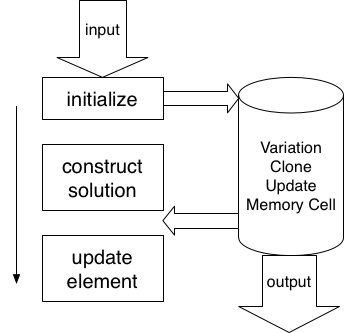
\includegraphics[height=5cm]{img/flow-chart.png}
\caption{Flow Chart}
\end{figure}

\subsection{Term Definition}
\begin{itemize}
\item \textbf{Antigen}\\
In connected graph $G$ , starting from any vertex, all other vertices are accessed, each vertex is visited only once (except for start and end), and the sequence of vertices that constitutes the shortest path is defined as antigen $A_{g}$.

\item \textbf{Antibody}\\
In connected graph $G$ , starting from any vertex, all other vertices are accessed, each vertex is visited only once (except for start and end), and the sequence of vertices that constitutes the path is defined as antibody $A_{b}$. Antibody set is defined as:
\begin{equation}
D=\left \{\left \langle s,dist\right \rangle | s \in P , dist \in N \right \}
\tag{2}
\end{equation}
$s$ is the sequence loops of $n$ city nodes, and $dist$ is the length of loop path.

\item \textbf{Affinity}\\
Affinity measures the degree of match between an antibody and antigen. Here the affinity calculation uses a distance-based matching algorithm. Defining affinity between antibodies $A_{b}$ and antigens  $A_{g}$ as follows: 
\begin{equation}
f_{dist}\left(A_{b},A_{g} \right) = 1 /\left(A_{b}.dist - A_{g}.dist\right)
\tag{3}
\end{equation}
The greater the affinity of antibody for antigen, the closer the candidate solution is to optimal solution. But we currently don’t know the value of $A_{g}.dist$, so we need to give a parameter according to the scale of problem and the initial value of city distance, here gives a parameter $T$:
\begin{equation}
T = \left(\sum_{i=1}^{n} \sum_{j=1}^{n}d\left(i,j\right)\right)/\left(2n\right)
\tag{4}
\end{equation}
The affinity formula is modified to:
\begin{equation}
f_{dist}\left(A_{b},A_{g} \right) = 1 /\left(A_{b}.dist - T\right)
\tag{5}
\end{equation}

\item \textbf{Memory Cell}\\
Let the memory cell mean that the affinity between initial antibody and antigen exceeds the activation threshold, and the antibody is activated to evolve into a memory cell. Defined $M$ as a collection memory cells, as in Equation \ref {eq6}
\begin{equation}
M=\left \{ x |f_{dist} \left(A_{b},A_{g}\right)\geqslant \theta,x \in D \right \}
\tag{6} \label {eq6}
\end{equation}

\item \textbf{Path Transition Probability}\\
$p{_{ij}}^{k} $ indicates the probability that ant $k$ will be transferred from city $i$ to city $j$ at time $t$, calculated as follows:
\begin{equation}
p{_{ij}}^{k} =
\begin{cases}
\frac{[\tau_{ij}(t)]^\alpha \cdot [\eta_{ij}]^\beta} { \sum\limits_{s \subset allowed_{k}} [\tau_{is}(t)]^\alpha \cdot [\eta_{is}(t)]^\beta} & j \in allowed_k \\
0 & else
\end{cases}
\tag{7}
\end{equation}
Where $\tau_{ij}(t)$ represents the concentration of pheromone on edge $\left(i,j\right)$ at time $t$, $\eta_{ij}$ represents the visibility of edge $\left(i,j\right)$, denotes the expectation degree from city $i$ to $j$, indicates that the ant will allow the selected city $k$ in next step. $\alpha$ and $\beta$ separately indicate the relative importance of information and heuristic information accumulated by ants in the process of ant selection.
\end{itemize}

\subsection{Immune Clone Algorithm}
The clonal selection mechanism\upcite{Khilwani.2008} is a dynamic process adaptive to the immune system of organisms. The first part of the individuals with higher affinity produce clonal amplification and mutation, which promotes the further maturation of the affinity. The immune complementation mechanism maintains the diversity of antibodies and enables the antibodies to handle different In the form of antigens, the presence of immune memory allows excellent individuals and their information to be maintained.

The clonal selection mechanism in the algorithm embodies three steps in each iteration: cloning, mutation, and selection.
\begin{enumerate}
\item{ \textbf{Clone:} Corresponding to the biological immune immune response process, according to the size of the affinity of the immune memory cells and the antigen (problem), a positive-scale clonal antibody population is generated.}
\item{\textbf{Variation:} Individuals in resulting clonal population are mutated to form mutated individuals. The mutation consists of three sub-operators: first is to randomly intercept the cloned antibody,  second is to use the intercepted fragment, construct a new antibody using standard ant colony algorithm, and third is to change the gene position of the poorer individual.}
\item{\textbf{Selection:} The memory bank is updated based on the affinity of the variant antibody with respect to antigen.}
\end{enumerate}

\section{Algorithm Steps}
The hybrid algorithm based on immune ant colony has the rapidity and randomness of immune algorithm, generates effective initial information, and accelerates the search speed of the ant colony algorithm. However, in the later stage of the hybrid algorithm, since the search for the path with less pheromone is neglected during the selection of the path, the phenomenon of stagnation easily occurs. In order to overcome this phenomenon, by using the concentration suppression mechanism in the immune algorithm, the concept of path concentration is introduced in the ant colony algorithm, and the path selection probability is affected by adjusting the pheromone intensity expressed by the path to maintain the diversity of the ant colony. To avoid stagnation in the ant colony algorithm.The specific algorithm process is as follows.

\subsection{Feasible Solution}
Calculate a feasible solution using immune algorithm.
\begin{enumerate}
\item {Enter question and determine the antibody encoding}\\
The objective function and constraints of the input problem are used as antigens of immune algorithm. Antibodies are coded in natural numbers and one string represents one candidate solution.
\item {Calculate antibody affinity }\\
First calculate the affinity $f$ between the antibody $i$ and antigen $j$. The affinity exceeds threshold $\theta$ is activated and evolved into a memory cell.
\item{Antibody clone variation} \\
Detectors $A_{bj}$ in memory cells $M$ are clonally expanded to obtain antibody populations $C_{j}$ based on their affinity size, The more affinity antibodies, the more individuals that can replicate, the number of specific clones is calculated as:
\begin{equation}
i=INT[num \times \beta \div con]
\tag{8}
\end{equation}
In the formula, $INT$ is upper rounding function, $num$ is system-set clone size, $\beta$ is cumulative affinity of the antibody, $con$ is antibody concentration. The number of cloned antibodies is proportional to the cumulative affinity and inversely proportional to the antibody concentration. The higher the affinity of the antibody, the more effective the antibody is and the effective antibody clone should be stimulated. The higher antibody concentration indicates that the number of antibodies of the same species is too high. Due to limited system resources, cloning of such antibodies should be inhibited. Antibody concentration $con$ is calculated as:
\begin{equation}
con_i=\frac{M_{bi}}{M_{b}}
\tag{9} \label {eq9}
\end{equation}
 $|\cdot|$ indicates the number of collection elements,$M_{bi}$ is memory antibody subset that $id=i$, $M_{b}$ is whole memory antibody collection.
Do high frequency variation of $C_{j}$ to obtain antibody population $C_{j}^*$, the lower the antibody's affinity, the higher the mutation rate in $C_{j}$, and vice versa. The mutation rate is determined by Equation \ref {eq9}.

\item {Update group} \\
Select the mature detector $A_{bj}^*$ which has the accumulative highest affinity in $C_{j}^*$, if the affinity of $A_{bj}^*$ to $A_{gj}$ is higher than $A_{b}$, then use $A_{bj}^*$ to replace $A_{b}$ into the memory detector library.

\item{Terminal condition} \\
If the solution satisfy the termination condition and output a feasible solution; otherwise, go to step 2.

\end{enumerate}

\subsection{Initialize Pheromone}
Initialize the pheromone based on feasible solution.
According to the better feasible solution obtained by the previous algorithm, the initial distribution of pheromone is completed, the ant colony is placed on each node, and the initial value of the pheromone distribution is set as:
\begin{equation}
\tau_{ij}(0)=
\begin{cases}
\tau_C +\tau_G & (i,j)\\
\tau_C & else
\end{cases}
\tag{10}
\end{equation}
$\tau_G$ is a pheromone value obtained from a feasible solution solved by an immune algorithm, and calculated as Equation \ref {eq11}:
\begin{equation}
\tau_G = \frac{Q}{L^*}
\tag{11} \label {eq11}
\end{equation}
In the equation, $Q$ is the amount of information released by ant cycle in ant colony algorithm. $L^{*}$ is the optimal path length obtained by immune algorithm. The pheromone increment calculation formula of the ant colony algorithm is introduced into the calculation of the initial information amount, which is equivalent to predetermining the feasible solution obtained by the immune algorithm as a good path obtained in the ant colony algorithm. In this way, the ant colony algorithm can be run directly from a relatively good initial state, thus avoiding the initial redundant search of the algorithm.

\subsection{Probability Formula}
Construct probability formula using immune inhibition operators.
In the TSP problem, first put the edges passed into the collection $Tour$, Path concentration $C_{ij}$ is $e_{ij}$ the proportion of ant populations that have chosen path  in the ant colony to the size of the ant colony. 
\begin{equation}
C_{ij}(t) = \frac{1}{M} \sum\limits_{k=1}^{M}iif \left(e_{ij} \in Tour^k(t),1,0\right)
\tag{12}
\end{equation}
\par
In order to avoid overly concentrated edges on a certain edge or some paths from a certain node, it is necessary to dynamically control the concentration of the path during the construction of the solution. Thus, it is defined that during the $t$-th iteration, when ant $k$ constructs a solution from node $i$, the concentration of path $e_{ij}$ is:
\begin{equation}
C_{ij}^k(t) = \frac{1}{M} \sum\limits_{k=1}^{k-1}iif \left(e_{ij} \in Tour^k(t),1,0\right)
\tag{13}
\end{equation}
\par
Meanwhile, in order not to excessively concentrate the path selected by a certain ant, the pheromone represented by the edge is adjusted according to the concentration of the path. So we introduces the path expression pheromone $\tau_{ij}^k(t)$ at a certain moment, is a comprehensive representation of path concentration and path pheromone, defined as:
\begin{equation}
\tau_{ij}^k(t)=
\begin{cases}
\tau_{ij} \cdot \left(\lambda \cdot c_{ij}^k(t)\right) & if \quad c_{ij}^k(t) > c_0 \\
\tau_{ij} & else
\end{cases}
\tag{14}
\end{equation}
\par
The essence of expression pheromone is to scale and adjust the original pheromone value of the path, that is, to calibrate the pheromone based on the path concentration. When an ant selects a path, the larger the original pheromone of the path is, the larger the selection probability is, and vice versa. So expression pheromone will not only retain the high selectivity of edges with high original pheromone, but also reduce the pressure of choice on the same side, which creates a new diversity maintenance strategy. Based on this, the ant selection probability can be redefined as:
\begin{equation}
p{_{ij}}^{k} =
\begin{cases}
\frac{[\tau_{ij}^k(t)]^\alpha \cdot [\eta_{ij}]^\beta} { \sum\limits_{\mu \subset N^k_l(t)} [\tau_{i\mu}^k(t)]^\alpha \cdot [\eta_{i\mu}(t)]^\beta} & if \quad j \in N^k_i(t) \\
0 & else
\end{cases}
\tag{15}
\end{equation}

\subsection{Update Pheromone}
The pheromone local updating adopts the delay updating method, that is, after $n$($n$ represents the number of urban nodes) moments, after the ant completes a cycle, the pheromone on all the paths is locally updated according to Equation \ref {eq16}:
\begin{equation}
\tau_{ij}(t+n) = (1-\omega)\cdot\tau_{ij}(t)+\omega\cdot C
\tag{16} \label {eq16}
\end{equation}
In the formula, $\omega$ is a parameter between $0$ and $1$, $C$ is the given pheromone initial value.
At the same time, calculate the loop distance obtained by all ants in the loop, find the loop with shortest distance and longest distance, According to Equation \ref {eq17}, perform the global update on shortest loop’s and longest loop’s pheromone: 
\begin{equation}
\tau_{ij}(t+n) = (1-\rho)\cdot\tau_{ij}(t)+\rho\cdot \Delta{\tau_{ij}}'(t)
\tag{17} \label {eq17}
\end{equation}

\begin{equation}
\Delta{\tau_{ij}}'(t) = 
\begin{cases}
\frac{Q}{L_{best}} & e_{ij} \in L_{best} \\
-\frac{Q}{L_{worst}} & e_{ij} \in L_{worst} \\
0 & else
\end{cases}
\tag{18} \label {eq18}
\end{equation}

In the formula, $\rho$ is pheromone volatilization coefficient between 0 and 1, and $1-\rho$ denotes the persistence of pheromone preservation. $L_{best}$ is the length of shortest loop found by all ants in this cycle, $L_{worst}$ is the longest loop. Calculated according to Equation \ref {eq18} .

%--------------------------------------------------------------------------------
%Chapter4 Summary
%--------------------------------------------------------------------------------
\chapter{Summary}
The theoretical research of immune optimization algorithms can provide a solid foundation for the research of hybrid immune algorithms. There are two main types of hybrid of immune algorithms: one is to introduce the concept and mechanism of immunity into other algorithms, and use the diversity mechanism of antibodies to improve other algorithms, so that they can jump out of local extreme points and improve convergence and accuracy; Another is to introduce other algorithms into the immune algorithm, and overcome the shortcomings of the longer computation time of the immune algorithm, accelerate the convergence speed.

Due to the limitations and deficiencies to understand the complex biological immune systems with rich information processing mechanisms, the immune optimization algorithms inspired by biological immune systems also have great limitations; Most of immune algorithms theory learn from other heuristic algorithms such as genetic algorithms and artificial neural networks, the theoretical researches lag behind. Therefore, it is urgent to establish a mathematical theory system of unified immune algorithms. The improvement and perfection of the theoretical mechanism of the algorithm still need to be further studied in-depth.

Currently, the research of hybrid immune algorithms still stays in the simple accumulation of two or more optimization algorithms to a certain extent, and does not fully consider the inherent organic connections and essential differences between multiple optimization algorithms. Therefore, the research of hybrid immune algorithms still need to further develop to a deeper level: 
\begin{enumerate}
\item{In-depth analysis and mining of intelligent information processors in complex biological immune systems, and introducing more immune optimization mechanisms and algorithms into other more optimized methods.}
\item{Introduce more intelligent mechanisms such as co-evolution, chaos, and artificial endocrine mechanisms to immune algorithms, give full play to the advantages of each algorithm, and construct efficient hybrid immune algorithms to achieve a true fusion of immune algorithms and other optimization methods}
\end{enumerate}

%--------------------------------------------------------------------------------
%Reference
%--------------------------------------------------------------------------------
\appendix
\begin{thebibliography}{}
\bibitem {Holland.1992} 
Holland J H. Adaptation in natural and artificial systems: an introductory analysis with applications to biology, control, and artificial intelligence[M]. MIT press, 1992.
\bibitem {Forrest.1994} 
Forrest S, Perelson A S, Allen L, et al. Self-nonself discrimination in a computer[C]//Research in Security and Privacy, 1994. Proceedings., 1994 IEEE Computer Society Symposium on. Ieee, 1994: 202-212.
\bibitem {Tazawa.1997}
Tazawa I, Koakutsu S, Hirata H. An evolutionary optimization based on the immune system and its application to the VLSI floorplan design problem[J]. IEEJ Transactions on Electronics, Information and Systems, 1997, 117(7): 821-828.
\bibitem {Jiao.2000} 
Jiao L, Wang L. A novel genetic algorithm based on immunity[J]. IEEE Transactions on Systems, Man, and Cybernetics-part A: systems and humans, 2000, 30(5): 552-561.
\bibitem {Kennedy.1995} 
Eberhart R, Kennedy J. A new optimizer using particle swarm theory[C]//Micro Machine and Human Science, 1995. MHS'95., Proceedings of the Sixth International Symposium on. IEEE, 1995: 39-43.
\bibitem {Parsopoulos.2009}  
Parsopoulos K E. Cooperative micro-particle swarm optimization[C]//Proceedings of the first ACM/SIGEVO Summit on Genetic and Evolutionary Computation. ACM, 2009: 467-474.
\bibitem {Ratnaweera.2004}
Ratnaweera A, Halgamuge S K, Watson H C. Self-organizing hierarchical particle swarm optimizer with time-varying acceleration coefficients[J]. IEEE Transactions on evolutionary computation, 2004, 8(3): 240-255.
\bibitem {Ling.2008}
Ling S H, Iu H H C, Chan K Y, et al. Hybrid particle swarm optimization with wavelet mutation and its industrial applications[J]. IEEE Transactions on Systems, Man, and Cybernetics, Part B (Cybernetics), 2008, 38(3): 743-763.
\bibitem {Potter.1994}
Potter M A, De Jong K A. A cooperative coevolutionary approach to function optimization[C]//International Conference on Parallel Problem Solving from Nature. Springer, Berlin, Heidelberg, 1994: 249-257.
\bibitem {Vermaas.2009}  
Vermaas L L G, Honorio L M, Freire M, et al. Learning Fuzzy Systems by a Co-Evolutionary Artificial-Immune-Based Algorithm[C]//International Workshop on Fuzzy Logic and Applications. Springer, Berlin, Heidelberg, 2009: 312-319.
\bibitem {Dorigo.1996}
Dorigo M, Maniezzo V, Colorni A. Ant system: optimization by a colony of cooperating agents[J]. IEEE Transactions on Systems, Man, and Cybernetics, Part B (Cybernetics), 1996, 26(1): 29-41.
\bibitem {Qin.2006}
Qin L, Chen Y, Luo J, et al. Diversity Guaranteed Ant Colony Algorithm Based on Immune Strategy[C]//Computer and Computational Sciences, 2006. IMSCCS'06. First International Multi-Symposiums on. IEEE, 2006, 2: 217-223.
\bibitem {Ahuja.2007}
Ahuja A, Das S, Pahwa A. An AIS-ACO hybrid approach for multi-objective distribution system reconfiguration[J]. IEEE transactions on power systems, 2007, 22(3): 1101-1111.
\bibitem {Lu.2011}
Lu J, Wang N, Chen J, et al. Cooperative path planning for multiple UCAVs using an AIS-ACO hybrid approach[C]//Electronic and Mechanical Engineering and Information Technology (EMEIT), 2011 International Conference on. IEEE, 2011, 8: 4301-4305.
\bibitem {Jiao.2008}
Jiao L, Li Y, Gong M, et al. Quantum-inspired immune clonal algorithm for global optimization[J]. IEEE Transactions on Systems, Man, and Cybernetics, Part B (Cybernetics), 2008, 38(5): 1234-1253.
\bibitem {Solak.2012}
Solak K, Rebizant W, Klimek A. Fuzzy adaptive transmission-line differential relay immune to CT saturation[J]. IEEE Transactions on Power Delivery, 2012, 27(2): 766-772.
\bibitem {Liu.2012}
Liu H, Wu G, Wang T, et al. Optimizing fracturing design with a RBF neural network based on immune principles[C]//Cognitive Informatics \& Cognitive Computing (ICCI* CC), 2012 IEEE 11th International Conference on. IEEE, 2012: 336-340.
\bibitem {Khilwani.2008}
Khilwani A. Fast colonel algorithm[J]. Engineering Applications of Artificial Intelligence, 2008, 21(1):106 -128.
\end{thebibliography}

\end{document}


